\documentclass[../report.tex]{subfiles}
\begin{document}
    
    \begin{frame}
        \frametitle{4a: Hierarchical LK}
        \begin{figure}[!htb]
            \centering
            \frame{
\includegraphics[keepaspectratio,height=0.65\textheight,width=0.45\textwidth]{ps4-4-a-1}}
            \caption{ps4-4-a-1}
        \end{figure}
    \end{frame}

    \begin{frame}
        \frametitle{4a: Hierarchical LK (cont.)}
        \begin{figure}[!htb]
            \centering
            \frame{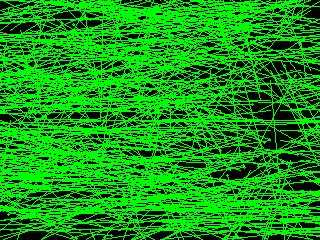
\includegraphics[keepaspectratio,height=0.65\textheight,width=0.45\textwidth]{ps4-4-a-2}}
            \caption{ps4-4-a-2}
        \end{figure}
    \end{frame}

    \begin{frame}
        \frametitle{4a: Hierarchical LK (cont.)}
        \begin{figure}[!htb]
            \centering
            \frame{
\includegraphics[keepaspectratio,height=0.65\textheight,width=0.45\textwidth]{ps4-4-a-3}}
            \caption{ps4-4-a-3}
        \end{figure}
    \end{frame}

    \begin{frame}
        \frametitle{4b: Hierarchical LK (cont.)}
        \begin{figure}[!htb]
            \centering
            \frame{
\includegraphics[keepaspectratio,height=0.65\textheight,width=0.45\textwidth]{ps4-4-b-1}}
            \caption{ps4-4-b-1}
        \end{figure}
    \end{frame}

    \begin{frame}
        \frametitle{4b: Hierarchical LK (cont.)}
        \begin{figure}[!htb]
            \centering
            \frame{
\includegraphics[keepaspectratio,height=0.65\textheight,width=0.45\textwidth]{ps4-4-b-2}}
            \caption{ps4-4-b-2}
        \end{figure}
    \end{frame}
    
\end{document}